\section{Approach to Solving \gls{rsp}s}

This section presents a heuristic algorithm to safely solve a robust signomial program based on our previous discussion on robust geometric programming. 

\subsection{General RSP Solver}
As mentioned before, a common heuristic algorithm to solve an SP is by sequentially solving local GP approximations, but the solution is not guaranteed to be globally optimal. Our approach to solve an RSP is based on sequentially solving local RGP approximations. Below we provide a step-by-step algorithm to solve an RSP:

\begin{enumerate}
    \item Choose an initial guess $x_0$
    \item Repeat
    \begin{enumerate}
        \item Find the local GP approximation of the SP at $x_i$.
        \item Find the RGP formulation of the GP.
        \item Solve the RGP to obtain $x_{i+1}$.
        \item If $x_{i+1} \approx x_{i}$: break
    \end{enumerate}
\end{enumerate}

Similar to an SP, a good initial guess would lead to faster convergence and possibly a better solution. A quick candidate is the deterministic solution of the uncertain SP, which will certainly lead to a faster convergence.

\begin{figure}[h]
    \centering
    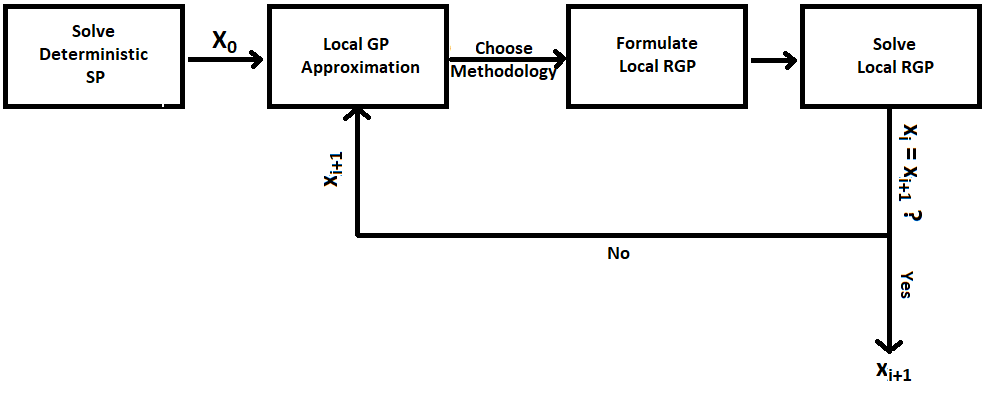
\includegraphics[scale=0.6]{sp_solve.png}
    \caption{A block diagram showing the steps of solving an RSP}
    \label{fig:solve_rsp_diag}
\end{figure}

Any of the previously mentioned methodologies can be used to formulate the local RGP approximation. 
However, Depending on the RGP formulation chosen to solve an RSP, the last two blocks in Figure \ref{fig:solve_rsp_diag} are tweaked slightly for a faster convergence. 
\ \\
\subsection{Best Pairs RSP Solver}
If the Best Pairs methodology is exploited, then the above algorithm would change so that each iteration would solve the local RGP approximation and choose the best permutation for each large posynomial. The modified algorithm would become as follows:

\begin{enumerate}
    \item Choose an initial guess $x_0$
    \item Repeat
    \begin{enumerate}
        \item Find the local GP approximation of the SP at $x_i$.
        \item $\forall (i,j) \in \mathbf{P}$, select the new permutations $\phi \in \hat{\mathcal{P}}_{i,j}$ such that $\phi$ minimizes $\textstyle{\sum}_{k=1}^{|S_{i,j}|/2} {\displaystyle \max_{\vec{\zeta} \in \mathcal{Z}}} \left\{e^{\mathcal{L}^{\phi_{2k-1}}_{i,j}} + e^{\mathcal{L}^{\phi_{2k}}_{i,j}}\right\}\bigg\rvert_{\vec{x}_i}$
        \item Solve the approximate tractable counterparts of the local GP in \eqref{GP_counterparts_tractable}, and let $\vec{x}_{i+1}$ be the solution
        \item If $x_{i+1} \approx x_{i}$: break
    \end{enumerate}
\end{enumerate}

\subsection{Linearized Perturbations RSP Solver}
On the other hand, if the Linearized Perturbations formulation is to be used, then we can avoid solving a signomial program at each iteration by first approximating the original SP constraints locally, and in the same loop approximating the robustified possibly signomial constraints locally, thus solving a GP at each iteration instead of an SP. The algorithm would then become as follows:

\begin{enumerate}
    \item Choose an initial guess $x_0$
    \item Repeat
    \begin{enumerate}
        \item Find the local GP approximation of the SP at $x_i$.
        \item Robustify the constraints of the local GP approximation using the Linearized Perturbations methodology.
        \item Find the local GP approximation of the resulting local SP at $x_i$.
        \item Solve the local GP approximation in step c to obtain $x_{i+1}$
        \item If $x_{i+1} \approx x_{i}$: break
    \end{enumerate}
\end{enumerate}
